\documentclass[a4paper,11pt]{jsarticle}
% !TEX encoding = UTF-8

\usepackage[dvipdfmx]{hyperref}
\usepackage{pxjahyper}


% 数式
\usepackage{amsmath,amsfonts}
\usepackage{bm}
\usepackage{physics}
\usepackage{amsmath,amssymb}
\usepackage{mathtools}
\numberwithin{equation}{section}

% 画像
\usepackage[dvipdfmx]{graphicx}
\usepackage{ascmac}

\usepackage{url}
\usepackage[dvipdfmx]{hyperref}

% \e と \i を定義
\providecommand{\e}{\mathrm{e}}
\renewcommand{\i}{\mathrm{i}}

\begin{document}

\title{エニオン}
\author{T.S.}
\date{\today}
\maketitle
\tableofcontents


以下の議論はNathan M. Myers "Thermodynamics of Statistic Anyons"を根幹に添え、T.S.による正しいかわからない考察を含む。\\

\section{Hong-Ou-Mandel効果}
HOM効果は量子光学で見つかった効果である。これを用いることによって、エニオニックな波動関数を作ることができる。\\
まず、HOM効果について復習しよう。2つのポートに、エンタングルしている光子のペアが対称的に入射する。
周波数や偏光状態などの自由度は同じとする。
初期状態がボソニックな空間部分の波動関数は、それぞれのインプットの重ね合わせで得られ、

\begin{align}
\ket{\psi_i^B}=\frac{1}{\sqrt{2}}(\ket{a}_1\ket{b}_2+\ket{b}_1\ket{a}_2)
\end{align}

となる。ビームスプリッタの作用は、状態を

\begin{align}
\ket{a}\to\frac{1}{\sqrt{2}}(\ket{c}+i\ket{d})\\
\ket{b}\to\frac{1}{\sqrt{2}}(i\ket{c}+\ket{d})
\end{align}

と変える。反射の際に、$\pi$の位相を獲得することが、変化の際の虚部に反映されていることに注意。
粒子のインデックスを追跡しながら、各インプットの状態についてこの発展を行うと、同じポートにいく状態のみが残ることがわかる:

\begin{align}
\ket{\psi_i^B}\to\ket{\psi_f^B}=\frac{i}{\sqrt{2}}(\ket{c}_1\ket{c}_2+\ket{d}_1\ket{d}_2)
\end{align}

物理的にはこれは有効的なボソン間の引力の現れとみれる(典型的には、”ボソンバンチング”と呼ばれる)。
\url{https://pc.watch.impress.co.jp/docs/news/yajiuma/754016.html} により、実験的にもわかっている。

\section{内部自由度を考慮したHOM効果}
フォトンの内部自由度を追加してHOM効果を拡張しよう。
フォトンをベル状態で用意することを考える。
4つの可能なベルペアは

\begin{align}
\ket{\Phi_A}=\frac{1}{\sqrt{2}}(\ket{00}+\ket{11})\\
\ket{\Phi_B}=\frac{1}{\sqrt{2}}(\ket{00}-\ket{11})\\
\ket{\Phi_C}=\frac{1}{\sqrt{2}}(\ket{01}+\ket{10})\\
\ket{\Phi_D}=\frac{1}{\sqrt{2}}(\ket{01}-\ket{10})\\
\end{align}

である。ここで、$\ket{0},\ket{1}$は直交する偏光状態である。
この追加の自由度を利用して、フェルミオンの、究極的にはエニオン的な統計量をフォトンにふるまいに組み込める。
このような使い方で、フォトンは”量子基板”と考えられる。\\
ここで、$\ket{\Phi_i},i=A,B,C$は対称的であり、$\ket{\Phi_D}$は反対称的であることに注意しよう。
フォトンはボソンであるから、全体の波動関数は対称的でなければならない。
よって、全体の波動関数としては2種類のパターンが考えられる。\\
ひとつめは

\begin{align}
  \ket{\Psi_i^B}=\frac{1}{\sqrt{2}}(\ket{a}_1\ket{b}_2+\ket{b}_1\ket{a}_2)\otimes\ket{\Phi_j},\,j=A,B,C
\end{align}

であり、ふたつめは

\begin{align}
  \ket{\Psi_i^F}=\frac{1}{\sqrt{2}}(\ket{a}_1\ket{b}_2-\ket{b}_1\ket{a}_2)\otimes\ket{\Phi_D}
\end{align}

である。無偏光状態を仮定すると、ビームスプリッタは波動関数の空間部分のみに作用する。
後者の場合、アウトプット状態は

\begin{align}
  \ket{\Psi_i^F}\to\ket{\Psi_f^F}=\frac{1}{\sqrt{2}}(\ket{c}_1\ket{d}_2-\ket{d}_1\ket{c}_2)
\end{align}

となり、フォトンのペアはお互いに異なるポートに向かうことになる。
これは有効的には、フェルミオン間の引力が働くということを示しており、パウリの排他律のあらわれであるとみれる。
フォトンは原理的にはボソンであるにもかかわらず、ビームスプリッタが反対称な部分のみにアクセスするため、フォトンはフェルミオンのようにふるまう。

\begin{figure}[htbp]
  \begin{center}
  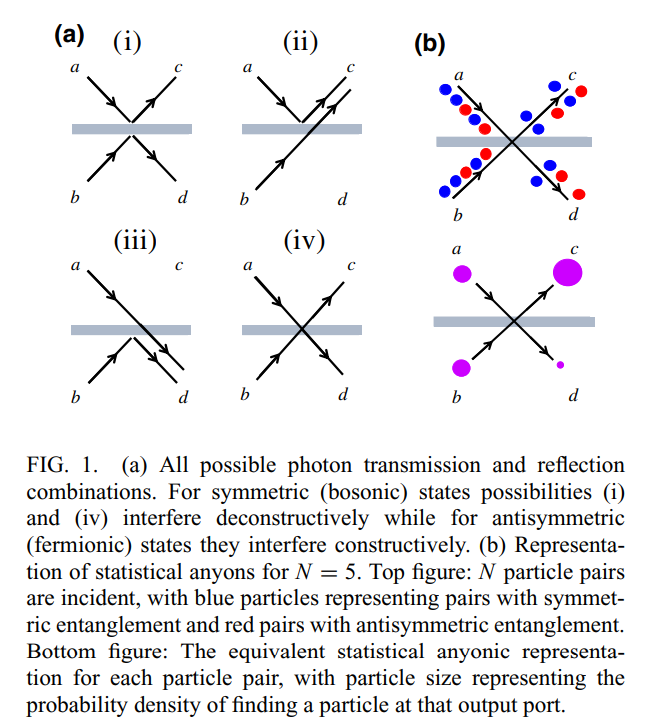
\includegraphics[width=100mm]{fig1.png}
  \caption{HOM効果の結果}
  \end{center}
  \end{figure}
  


\section{Hong-Ou-Mandel効果でエニオンの波動関数を作る}
このHOM効果は、対称or反対称のベル状態を調整することにより、エニオニックな統計に拡張できる。
偏光を回転させたビームスプリッタを使ったり、導波路を調整したり、偏光版を入れることにより、位相をコントロールできる。
対称と反対称にエンタングルしたペアを統計的に混ぜて用意してみよう:

\begin{align}
  \ket{\psi_i^A} = \frac{1}{\sqrt{2}} \left( \ket{a}_1 \ket{b}_2 + \mathrm{e}^{\i \pi \nu} \ket{b}_1 \ket{a}_2 \right)
\end{align}

\subsection{元論文(8)の結果を計算してみる}
昨日の議論のなかで、藤井先生から$\ket{\Psi_i^B,\ket{\Psi_i^F}}$をそれぞれ$\cos(\pi\nu)=\cos{\theta},\mathrm{i}\sin{\theta}$で重みづけして計算してみると元論文(8)となるのでは、という意見をいただいたので、その方針で計算をしてみる。
結果的には、まだ上手くいっていないので、上手くいかない理由を説明するため、もっと一般の方法により計算を記述してみる。\\

\begin{itembox}[l]{\textbf{(8)の計算 }}
$\ket{\Psi_i^B},\ket{\Psi_i^F}$をそれぞれ$x,y \in \mathbb{C}$で重みづけして足す。ここで、$|x+y|=1$である。
\end{itembox}
<計算はじめ>
\begin{align}
x\ket{\Psi_i^B}+y\ket{\Psi_i^F} &= \frac{x}{2}(\ket{a}\ket{b}+\ket{b}\ket{a})\otimes (\ket{01+\ket{10}})+\frac{y}{2}(\ket{a}\ket{b}-\ket{b}\ket{a})\otimes (\ket{01-\ket{10}})\\
&=\frac{1}{2}[(x+y)\ket{a}\ket{b}+(x-y)\ket{b}\ket{a}]\otimes\ket{01} \notag\\
&\,\,\,\,  +\frac{1}{2}[(x-y)\ket{b}\ket{a}+(x+y)\ket{b}\ket{a}]\otimes\ket{10}\\
&=\frac{1}{2}[(x+y)\ket{a}\ket{b}+(x-y)\ket{b}\ket{a}]\otimes\ket{01} \notag\\
&\,\,\,\, +\left(\frac{(x-y)^2}{x+y}\ket{a}\ket{b}+(x-y)\ket{b}\ket{a}\right)\otimes\frac{x+y}{x-y}\ket{10} 
\end{align}
となる。
ここで、
\begin{itembox}[l]{\textbf{Assumption}}
  $x,y$について、
  \begin{align}
  \frac{(x-y)^2}{x+y}=x+y
  \end{align}
を満たすとする。
\end{itembox}
このとき、計算結果はまとめられることになる:

\begin{align}
  x\ket{\Psi_i^B}+y\ket{\Psi_i^F} &=
  \frac{1}{2}[(x+y)\ket{a}\ket{b}+(x-y)\ket{b}\ket{a}]\otimes\ket{01} \notag\\
  &\,\,\,\,+\left(\frac{(x-y)^2}{x+y}\ket{a}\ket{b}+(x-y)\ket{b}\ket{a}\right)\otimes\frac{x+y}{x-y}\ket{10} \\
  &=\frac{1}{2}\left[(x+y)\ket{a}\ket{b}+(x-y)\ket{b}\ket{a}\right]\otimes\left[\ket{01}+\frac{x+y}{x-y}\ket{10}\right]\\
  &=\frac{x+y}{2}\left[\ket{a}\ket{b}+\frac{x-y}{x+y}\ket{b}\ket{a}\right]\otimes\left[\ket{01}+\frac{x+y}{x-y}\ket{10}\right]
\end{align}

2つ目の=では、仮定を用いている。
(3.6)が、一般的な結果であり、形をまとめるうえでは仮定が必要となる。
ではここで、仮定が妥当であるか考えていく。\\

\begin{itembox}[l]{\textbf{仮定の検証}}
  仮定(3.5)は、
  \begin{align}
    \frac{(x-y)^2}{x+y}=x+y
  \end{align}
  という式である。これを変形すると、
  \begin{align}
    (x-y)^2=(x+y)^2
  \end{align}
  となる。これは、
  \begin{align}
    x^2-2xy+y^2=x^2+2xy+y^2
  \end{align}
  となる。これを整理すると、
  \begin{align}
    4xy=0
  \end{align}
  となる。これは、$x,y$のどちらかが0であることを意味する。
  よって、0でない方は1となり、これはそれぞれを有限の割合で足し合わせるという、やりたいこととは異なる。
  したがって、この仮定は妥当でない。
\end{itembox}

以上の結果から、元論文(8)の計算は、上手くいっていないため、どこで間違えたか考える必要がある。
元論文(8)式は内部自由度の波動関数が記述されていないことから、どこかのひと部分のみの記述をしているなどであろうか?
((8)についての補足終了)\\

\subsection{論文の続き}

エニオニックな波動関数が(3.1)であることを認めて進めていく。
この波動関数は、ビームスプリッタの作用によって、

\begin{align}
  \ket{\psi_i^A} \to \ket{\psi_f^A}=\frac{1}{2\sqrt{2}}\left[(\ket{c}_1+i\ket{b}_1)(\ket{d}_2+i\ket{c}_2)+\mathrm{e}^{i\pi\nu}(\ket{d}_1+i\ket{c}_1)(\ket{c}_2+i\ket{d}_2)\right]
\end{align}
と発展する。
これを用いることにより、両方の光子が同じ方に来る確率は

\begin{align}
  P_{\mathrm{same}} &= P_C+P_D \\
  &= |\bra{c}_1\bra{c}_2\ket{\psi_f^A}|^2+|\bra{d}_1\bra{d}_2\ket{\psi_f^A}|^2\\
  &=\frac{1}{2}[1+\cos(\pi \nu)] &&
\end{align}


と計算できる。\\
$\nu$ が様々な値をとるため、$P_{\mathrm{same}}$ は0から1まで値をとる。$N$個の光子をある割合で対称的にエンタングルさせ、残りは反対称にエンタングルさせたとする。
このときは、対称的or反対称的にエンタングルしているペアの分布をただ変えるだけでその振る舞いが反映される(平均的に)。
このフレームワークの中で、$\nu$はあるペアが対称的にエンタングルしている確率の尺度となる。すなわち、$\nu=\nu(p_B)$である。\\

\begin{itembox}[l]{\textbf{Def.エニオンの分類}}
多数のエニオンについて、統計的に$\nu=\nu(p_B)$の性質を持つエニオンを統計エニオンと呼ぶ。\\
対照的に、Wilczekの電荷と磁束の思考によるエニオンをトポロジカルエニオンと呼ぶ。したがって、分数量子ホール効果における準粒子励起もトポロジカルエニオンである。
\end{itembox}

多数ある粒子の平均として、ボソンとフェルミオンの中間のような性質をもつのが統計エニオンであって、準粒子そのものの性質として入れ替えの際に位相を得るのがトポロジカルエニオンであることに注意せよ。
また、トポロジカルエニオンといったときには、ここでは可換エニオンを考えることにする。可換エニオンとは、粒子の入れ替えにおいて単純に位相$\mathrm{e}^{i\pi\nu}$を得る粒子である。

トポロジーの立場に立てば、統計エニオンとトポロジカルエニオンの間には重要な区別が存在する。\\
トポロジカルエニオンの統計はブレイド(組みひも)群の表現である。(フェルミオンとボソンは置換群である。)
これは、2次元であることに起因しており、2回の粒子入れ替えが、何もしていないこととトポロジカルに区別しなくてはいけないというということである。
3次元では、2回の粒子入れ替えとなにもしないのとはトポロジカルに同等である。\\
これは物理的には、交換の方向が重要という結果を導く。2回同じ方向に入れ替えると、元の位相から$\mathrm{e}^{2i\pi \nu}$だけ変わる。\\
統計エニオンは、ボソンとフェルミオンの混合の平均であるから、2つの連続した交換は、交換の方向によらず、同じ波動関数に戻る。
混合の任意のペアをもってきたときの平均の位相はボソニックな位相とフェルミオニックな位相の平均である。すなわち、-1から1の間をとる。
ゆえに、位相$\mathrm{i\pi \nu}$をもつトポロジカルエニオンの混合に対応する統計エニオンは、混合の位相の平均が$cos(\pi \nu(p_B))$であるように重みづけされる。
我々は、可能なトポロジカルエニオンの位相を2次元空間を円とみる。ボソニックな位相とフェルミオニックな位相は正反対の位置として表現できる。
統計エニオンの平均された位相の可能な空間は、円の直径の線上で表現される。\\

この幾何学的な見方では、統計エニオンの平均された位相は対応するトポロジカルエニオンの位相の実数軸への角への射影とみなせる。(?)
図2がこの見方の図である。
この比較から、ブレイド群の表現として、トポロジカルエニオンは統計エニオンより複雑であることがわかる。
ここで、トポロジカルエニオンと統計エニオンの熱力学的な性質はどのように異なるか気になるだろう。から、次からその話を始めよう。

\section{統計エニオンの波動関数}
量子光学での知見から、統計エニオンを考えてみる。ボソニックな粒子のペアの波動関数の空間部分(内部自由度を除いた部分のこと)は

\begin{align}
\Psi_B(x,y) = \frac{1}{\sqrt{2(1+\delta_{n_1,n_2})}}[\psi_{n1}(x)\psi_{n2}(y)+\psi_{n1}(y)\psi_{n2}(x)]
\end{align}

ここで$\psi_n(x)$は量子数$n$に対応する規格化された1粒子固有状態である。規格化係数は、2粒子が同じときと違うときで変わる。区別できる2粒子のとき、因子2がかかる。
これは古典的な場合にかかる因子と同じである。
同様にフェルミオニックな波動関数は

\begin{align}
  \Psi_F(x,y) = \frac{1}{\sqrt{2}}[\psi_{n1}(x)\psi_{n2}(y)-\psi_{n1}(y)\psi_{n2}(x)]
\end{align}

フェルミオニックな波動関数のときは、規格化係数に$\delta$関数は必要ない。←これはなぜ?\\
$N$個の独立な粒子のペアについて、$N_B$個のペアが交換の際に対称的で、$N-N_B$個が反対称的であるとすると、

\begin{align}
\Psi(\vb*{x_1},\vb*{x_2},...,\vb*{x_N})=\prod_{j=1}^{N_B}\Psi_B(\vb*{x}_j)\prod_{k=N_B+1}^{N}\Psi_F(\vb*{x}_k)
\end{align}

となる。ここで、$\vb*{x_i}=(x,y)$である。
そしてこれは、統計エニオンの枠組みにおいて、次の式と等価である:

\begin{align}
  \Psi(\vb*{x_1},\vb*{x_2},...,\vb*{x_N})=\prod_{j=1}^{N}\Psi_A(\vb*{x}_j)
\end{align}

ここで、

\begin{align}
\Psi_A(\vb*{x}_j)&=\frac{1}{\sqrt{2(1+\delta_{n_1,n_2})}}[\psi_{n1}(x_j)\psi_{n2}(y_j)+\mathrm{e}^{i\pi\nu_j}\psi_{n1}(y_j)\psi_{n2}(x_j)]\\
\end{align}

である。

\subsection{元論文(13)から(12)を導く}
$\nu_j=\Theta(j-N_B-1)$のとき、元論文の(13)式から(12)式が導ける。
\begin{align}
  \Psi(\vb*{x_1},\vb*{x_2},...,\vb*{x_N})&=\prod_{j=1}^{N}\Psi_A(\vb*{x}_j)\\
  &=\prod_{j=1}^{N}\frac{1}{\sqrt{2(1+\delta_{n_1,n_2})}}[\psi_{n1}(x_j)\psi_{n2}(y_j)+\mathrm{e}^{i\pi\nu_j}\psi_{n1}(y_j)\psi_{n2}(x_j)]\\
  &=\prod_{j=1}^{N}\frac{1}{\sqrt{2(1+\delta_{n_1,n_2})}}[\psi_{n1}(x_j)\psi_{n2}(y_j)+\mathrm{e}^{i\pi\Theta(j-N_B-1)}\psi_{n1}(y_j)\psi_{n2}(x_j)]\\
  &=\prod_{j=1}^{N_B}\frac{1}{\sqrt{2(1+\delta_{n_1,n_2})}}[\psi_{n1}(x_j)\psi_{n2}(y_j)+\psi_{n1}(y_j)\psi_{n2}(x_j)]\notag\\
  &\times\prod_{k=N_B+1}^{N}\frac{1}{\sqrt{2(1+\delta_{n_1,n_2})}}[\psi_{n1}(x_k)\psi_{n2}(y_k)+\mathrm{e}^{i\pi}\psi_{n1}(y_k)\psi_{n2}(x_k)]\\
  &=\prod_{j=1}^{N_B}\frac{1}{\sqrt{2(1+\delta_{n_1,n_2})}}[\psi_{n1}(x_j)\psi_{n2}(y_j)+\psi_{n1}(y_j)\psi_{n2}(x_j)]\notag\\
  &\times\prod_{k=N_B+1}^{N}[\psi_{n1}(x_k)\psi_{n2}(y_k)-\psi_{n1}(y_k)\psi_{n2}(x_k)]\\
  &=\prod_{j=1}^{N_B}\Psi_B(\vb*{x}_j)\prod_{k=N_B+1}^{N}\Psi_F(\vb*{x}_k) 
\end{align}

より、導かれた。ここで、$\Theta(j-N_B-1)$はHeavisideの階段関数であることを用いた。

\subsection{論文の続き}
これをみると、統計エニオンは1粒子波動関数の積から成り立っていることがわかる。一方、トポロジカルエニオンの波動関数は一般に、エニオニックな位相のボソニック、フェルミオニックな極限を除いて、一粒子波動関数の積にはならないことに注意。
統計エニオンの波動関数内の積は、$N_B$個の対称な波動関数と$N_F$個の波動関数を与えなければならない。
この条件は、$\nu_j=\Theta(j-N_B-1)$となるとき満たされる。ここで、$\Theta(・)$はHeavisideの階段関数である。$\Theta(0)=1$としている。
このフレームワークでは、$\Psi_A(\vb*{x}_j)$のエニオニックな位相因子($\mathrm{e}^{i\pi\nu_j}$)は$N$個の粒子のペアのあらゆる交換の平均として考えられる。
大きな$N$については、$N_B=Np_B,N_F=N(1-p_B)$として表現できる。ここで、$p_B(p_F)$はペアがボソニック(フェルミオニック)な位相を持つ確率である。
この章の最後に、2粒子系の極限を考えてみよう。このとき、エニオニックな波動関数は

\begin{align}
  \Psi_A(\vb*{x})=\frac{1}{\sqrt{2(1+\delta_{n_1,n_2})}}[\psi_{n1}(x)\psi_{n2}(y)\pm \psi_{n1}(y)\psi_{n2}(x)]
\end{align}

ここで、符号は$p_B$が0か1かで決まる。個々のペアはボソンかフェルミオンかのどちらかであるということを反映している。

\section{統計エニオンの第二量子化}
適切な交換関係を決めることによって、統計エニオンは第二量子化をすることができる。

\subsection{トポロジカルエニオンの第二量子化}
まずトポロジカルエニオンについて考えよう。トポロジカルエニオンの生成消滅演算子については、ボソニックまたはフェルミオニックな演算子のJordan-Wigner変換(なんだこれ?)から作られる:
\\

\begin{itembox}[l]{\textbf{Def.トポロジカルエニオンの生成消滅演算子 }}
$\mathcal{C}$を交換のために回す方向で考える閉曲線とする。$a(\vb*{x}_\mathcal{C}),a^{\dag}(\vb*{x}_\mathcal{C})$を$\mathcal{C}$に沿った$\vb*{x}$の消滅,生成演算子とする。
このとき、トポロジカルエニオンの交換関係は次で与えられる。
\begin{align}
a(\vb*{x}_\mathcal{C})a(\vb*{y}_\mathcal{C})-\mathrm{e}^{-i\pi\nu}a(\vb*{y}_\mathcal{C})a(\vb*{x}_\mathcal{C})=0\\
a(\vb*{x}_\mathcal{C})a^{\dag}(\vb*{y}_\mathcal{C})-\mathrm{e}^{i\pi\nu}a^{\dag}(\vb*{y}_\mathcal{C})a(\vb*{x}_\mathcal{C})=0\\
a^{\dag}(\vb*{x}_\mathcal{C})a(\vb*{y}_\mathcal{C})-\mathrm{e}^{i\pi\nu}a(\vb*{y}_\mathcal{C})a^{\dag}(\vb*{x}_\mathcal{C})=0\\
a^{\dag}(\vb*{x}_\mathcal{C})a^{\dag}(\vb*{y}_\mathcal{C})-\mathrm{e}^{-i\pi\nu}a^{\dag}(\vb*{y}_\mathcal{C})a^{\dag}(\vb*{x}_\mathcal{C})=0
\end{align}
\end{itembox}

すなわち、生成同士、消滅同士の交換にはマイナスの位相がかかり、生成と消滅の交換にはプラスの位相がかかる。
トポロジカルエニオンの演算子はブレイド群の表現であるから、交換は時計回りか反時計回りかに依存する。(図1を参照。)
\begin{figure}[htbp]
\begin{center}
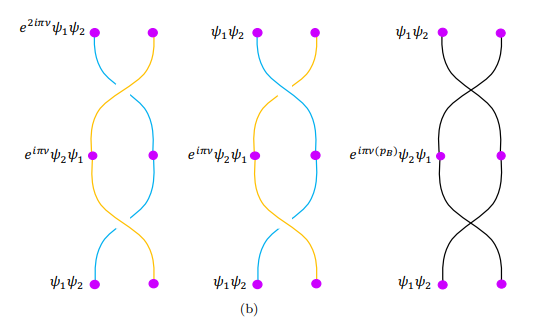
\includegraphics[width=100mm]{braidwf.png}
\caption{ブレイド}
\end{center}
\end{figure}

交換関係を見ると、$\nu=0$でボソンの交換関係を、$\nu=1$でフェルミオンの交換関係を復元することがわかる。
とくに、同じ位置にある粒子においては、エニオニックな位相はキャンセルされ、正準交換関係に帰着する:
\begin{align}
  a(\vb*{x}_\mathcal{C})a^{\dag}(\vb*{x}_\mathcal{C})\pm a^{\dag}(\vb*{x}_\mathcal{C})a(\vb*{x}_\mathcal{C})=1\\
\end{align}
ここで、エニオニックな演算子がフェルミオニックな演算子からきている場合は+、ボソニックな演算子からきている場合は$-$をとる。\\
一般に、トポロジカルエニオンは、$\nu\neq0$のとき、”ハードコアボソン”としてふるまう。ハードコアボソンとは、同じ位置にいない(排他律のある)ボソンである。
この意味で、$\nu$は2つの同一粒子の間の斥力の自由度を定量化していると考えられる。\\
ここの議論は\url{https://www.sciencedirect.com/science/article/pii/055032139390316H}{ A.Lerda, S.Sciuto. Anyons and Quantum Groups}による。

ハードコアボソンの生成消滅演算子$c_i^{\dag}(x_C),c_i(x_C)$を用いて、その議論を追ってみたい。
\begin{align}
  a(\vb*{x}_\mathcal{C})a^{\dag}(\vb*{x}_\mathcal{C})&=K_i(\vb*{x}_C)c_i(\vb*{x})c_i^{\dag}(\vb*{x})K_i^{\dag}(\vb*{x}_C)\\
  &=K_i(\vb*{x}_C)(-c_i^{\dag}(\vb*{x})c_i(\vb*{x})+1)K_i^{\dag}(\vb*{x}_C)\\
  &=-\mathrm{e}^{i\nu\Theta_C(\vb*{x},\vb*{x})}c_i^{\dag}(\vb*{x})K_i(\vb*{x}_c)\mathrm{e}^{i\nu\Theta_C(\vb*{x},\vb*{x})}K_i^{\dag}c_i(\vb*{x})+1\\
  &=-a_i^{\dag}(\vb*{x}_C)a_i(\vb*{x}_C)+1
\end{align}
ただし、
\begin{align}
 K_i(\vb*{x}_C)&=\mathrm{exp}(i\nu\sum_{y\in\Omega}\Theta_{c_{\vb*{x}}}(x,y)c_i^{\dag}(y)c_i(y))\\
K_i^{\dag}(\vb*{x}_C)&=c.c.=K_i^{-1}(\vb*{x}_c)
\end{align}
は、disorder演算子と呼ばれるものである。$\Omega,\Theta$はあとで定義を書くことにする。
これにより中途半端に示された。

\subsection{統計エニオンの第二量子化}
では次に、統計エニオンについて考えよう。
統計エニオンの生成消滅演算子を考えるには、統計エニオンの波動関数を構成したときを思い出せばよい。
量子多体系のHilbert空間として、Fock空間を考える。
そうすると、
\begin{align}
\ket{1}_1\ket{1}_2\dots\ket{1}_N=\prod _{j=1}^{N_B}b_j^{\dag}\ket{0}_j\prod _{k=N_B+1}^{N}f_k^{\dag}\ket{0}_k
\end{align}
と書くことができる。これと同等の表現として統計エニオンの生成演算子を考える:
\begin{align}
  \ket{1}_1\ket{1}_2\dots\ket{1}_N=\prod _{j=1}^{N}s_j^{\dag}\ket{0}_j
\end{align}
演算子$s_j^{\dag}$は、$j\leq N_B$ではボソンの生成演算子に、$N_B\leq j$ではフェルミオンの生成演算子にならなくてはならない。
同様に、消滅演算子も同じ条件を満たさなくてはならない。
この制限のもと、統計エニオンの交換関係は以下のようになる:\\

\begin{itembox}[l]{\textbf{Def.統計エニオンの交換関係 }}
  統計エニオンの交換関係は
\begin{align}
s_j^{\dag}s_j-\mathrm{e}^{i\pi\Theta(j-N_B-1)}s_j s_j^{\dag}=1\\
s_js_j^{\dag}-\mathrm{e}^{i\pi\Theta(j-N_B-1)}s_j^{\dag} s_j=1\\
s_j^{\dag}s_j^{\dag}-\mathrm{e}^{i\pi\Theta(j-N_B-1)}s_j^{\dag} s_j^{\dag}=0\\
s_js_j-\mathrm{e}^{i\pi\Theta(j-N_B-1)}s_j s_j=0
\end{align}
と定義する。
\end{itembox}

1粒子極限を考えると、生成演算子と消滅演算子の関係は

\begin{align}
s_js_j^{\dag}\pm s_j^{\dag}s_j=1
\end{align}

に帰着する。これは、現実にはボソンかフェルミオンかのどちらかであるということを反映している。
また、これは、(5)式の交換関係がフェルミオニックな演算子を元に作られたか、ボソニックな演算子を元に作られたかに依存することを反映している。

\section{統計エニオンと一般化排他統計(Generalized Exclusion Statistics)}
統計エニオンのフェルミオン極限を除いて、統計エニオンとトポロジカルエニオンの注目すべき違いは、排他律がないことである。
かわりに、統計エニオンは”部分的に占有された”状態を許す。
”部分的に占有された状態”というのは、全系の占有率が平均以上の状態である(?)。
この意味で、統計エニオンのフレームワークというのはHaldaneの一般化排他統計(Generalized Exclusion Statistics,GES)に似ている。\\
GESはパウリの排他律を拡張することによって作られたものである。
粒子数を変化させるもとで、量子系のHilbert空間の次元の変化を定量化するパラメタライズされた差分関係(differential relation)を定義することにより拡張された。(この文はまだよくわかっていないのでこんな感じ)
差分関係は

\begin{align}
\Delta  d_{GES}=-g \Delta  N
\end{align}

である。ここで左辺は次元の変化であり、$g$はパラメータだと考えられる。\\
ボソンに対しては、同じ状態を占められる粒子数は無限であるから、次元は粒子数に依存しない。よって$g=0$である。\\
フェルミオンに対しては、排他律のために、それぞれ、追加される粒子によって直接的に次元がスケールされる(粒子がいない次元は考えなくてよいということ?)。よって$g=1$である。\\
GES統計エニオンは、相互作用する気体、たとえばCalogero-Sutherlandモデルなどで見られることが示されている。
驚くべきことに、このGESエニオンの実現は、最低Landau準位に閉じ込められたトポロジカルエニオンに直接マッピングできる。
GESエニオンは、極低温Hubberdチェインと同様に、Calogero-SutherlandモデルやLieb-Linigerモデル、ハードコアTonks-Girardeau気体などに見られている。
もっと一般に、GESに従う理想準粒子の観点から、熱力学的Bethe仮設によって計算しなおせる可積分モデルの存在が示されている。\\
この統計エニオンのフレームワークでは、統計エニオンのHilbert空間の次元変化はボソンの次元変化とフェルミオンの次元変化の和で与えられる。
それぞれの出現確率$p_B,p_F$を用いて、
\begin{align}
\Delta d_{SA}=p_B\Delta d_b+p_F\Delta d_F
\end{align}
とかける。
$\Delta d_B=0,\Delta d_F=-\Delta N$のとき、$\Delta d_{SA}=-p_F\Delta N$と単純になる。
はじめの式と一つ上の式を見比べると、GESのフレームワークにおけるパラメータ$g$というのは、統計エニオンのフレームワークにおけるフェルミオンの出現確率によってきまってしまうということがわかる。
これは統計エニオンのフレームワークがGESエニオンのフレームワークとまったく同等であることを示している。
GESエニオンはボソンとフェルミオンの観点から説明できることは、MurthyとShankerが、Calogero-Sutherlandモデルは理想GESエニオンであることを指摘した際にわかった。
その結果、分配関数はボソニックな部分とフェルミオニックな部分に分けられ、それぞれ、GESパラメータ$g,g-1$の累乗で構成されることがわかった。
これにより、GESはボソンとフェルミオンの理想敵な混合であることが指摘された。\\
統計エニオン、GESエニオンは任意の次元で実現できる(次元に一般的な制限はない)というのは、トポロジカルエニオンとの大きな違いである。


\section{エニオンの平衡熱力学}
\subsection{1次元統計エニオン}
エニオン系の熱力学を理解するためにまず考えることは、熱力学量にエニオンの位相がどのように依存するかである。
これをきめるために、適切な分配関数を導入する。トラップされた相互作用するGESガスの実現でモチベートされたように、1次元調和ポテンシャル中の2つの統計エニオンを考えよう。\\
しかし、この際、我々は相互作用しない粒子系を考えている。
(GESは単なる混合でよいのか?)
トラップされたボソンーフェルミオン混合物は以前より、理論的あるいは実験的に研究されているが、この研究ではおもに、基底状態の設定でボソン、フェルミオン間の相互作用から生じる効果に焦点を当てよう。
統計エニオンのフレームワークでは我々は、混合物の代わりに、そのような混合の理想気体極限として多体平均のふるまいを考える。
調和ポテンシャル中に閉じ込められた2つの統計エニオンのハミルトニアンは

\begin{align}
H=\frac{p_1^2+p_2^2}{2m}+\frac{1}{2}m\omega^2(x_1^2+x_2^2)
\end{align}
で与えられる。統計エニオンののフレームワークでは、ハミルトニアンのもとで発展するエニオンのペアの分配関数というのは
\begin{align}
Z_{SA}=(Z_B)^{p_B}(Z_F)^{1-p_B}
\end{align}
となる。ここで、それぞれの粒子の分配関数を$Z_i,i=B,F$とした。
元論文の付録Aにはこの分配関数の導き方が書いてあるので余裕があるときに読む。$\rightarrow$ これを考えていく。

\subsection{調和ポテンシャル中の統計エニオンの分配関数}
  分配関数は次の様に定義される。ここで、$\ket{x_jy_j}$は位置の固有ケットである。
  \begin{align}
  Z_A^N=\mathrm{tr}{(\mathrm{e}^{-\beta H})}=\prod_{j=1}^N\int dx_j\int dy_j \bra{x_jy_j}\mathrm{e}^{-\beta H_j}\ket{x_j y_j}
  \end{align}
  ここで、
  \begin{align}
  H_j=\frac{p_{x_j}^2+p_{y_j}^2}{2m}+\frac{1}{2}m\omega^2(x_j^2+x_j^2)
  \end{align}
  である。エネルギー固有ケットをアイデンティティとして挟むことによって、位置表示の波動関数$\Psi_A(x_j,y_j)=\braket{n_1^{(j)}n_2^{(j)}}{x_jy_j}$を用いて、
  \begin{align}
  Z_A^N=\prod_{j=1}^N\int dx_j\int dy_j \sum _{n_1^{(j)},n_2^{(j)}} \sum _{m_1^{(j)},m_2^{(j)}} |\Psi_A(x_j,y_j)|^2 \\
  \times \mathrm{e}^{-\beta\hbar\omega(m_1^{(j)}+m_2^{(j)}+1)}\braket{n_1^{(j)}n_2^{(j)}}{m_1^{(j)}m_2^{(j)}} \notag 
  \end{align}
ここで、$\Psi_A(x_j,y_j)$は(4.5)式により定まり、ここでの$\psi$は調和ポテンシャル中の固有関数である。すなわち、
\begin{align}
\psi_n(x)=\frac{1}{\sqrt{2^n n!}}\left(\frac{m\omega}{\pi\hbar}\right)^{\frac{1}{4}}\mathrm{e}^{\frac{m\omega x^2}{2\hbar}}H_n\left(\sqrt{\frac{m\omega}{\hbar}}x\right)  
\end{align}
である($H_n$はエルミート多項式)。
エルミート多項式の直交性を利用することで、
\begin{align}
  Z_A^N=\prod_{j=1}^N \sum _{n_1^{(j)},n_2^{(j)}} \frac{1}{4}\mathrm{e}^{-\beta\hbar\omega(n_1^{(j)}+n_2^{(j)}+1)} \notag \\
  \times (2+\mathrm{e}^{-i\pi\Theta(j-N_B+1)}\delta_{n_1^{(j)},n_2^{(j)}}+\mathrm{e}^{i\pi\Theta (j-N_B+1)}\delta_{n_1^{(j)},n_2^{(j)}})  
\end{align}
積の記号をフェルミオンとボソンに分けることによって、
\begin{align}
  Z_A^N=\prod_{j=1}^{N_B}\sum_{n_1^{(j)},n_2^{(j)}=0}^{\infty}\frac{1}{2}\mathrm{e}^{-\beta\hbar\omega(n_1^{(j)}+n_2^{(j)}+1)}(1+\delta_{n_1^{(j)},n_2^{(j)}})\notag\\
  \times\prod_{k=N_B+1}^{N}\sum_{n_1^{(j)},n_2^{(j)}=0}^{\infty}\frac{1}{2}\mathrm{e}^{-\beta\hbar\omega(n_1^{(j)}+n_2^{(j)}+1)}(1-\delta_{n_1^{(j)},n_2^{(j)}})
\end{align}
これの初めの部分をボソンの分配関数、後半の部分をフェルミオンの分配関数として解釈することができる。
それゆえ、エニオニックな分配関数というのは、このように書ける。
\begin{align}
  Z_A^N=\prod_{j=1}^{N_B}Z_B^{(j)}\prod_{k=1}^{N_F}Z_F^{(k)}=Z_B^{N_B}Z_F^{N_F}=(Z_B^{p_B}Z_F^{p_F})^N
\end{align}
ここで、大きな$N$に対して、$p_B(p_F)$は粒子のペアがボソニック(フェルミオニック)な対称性をもつ確率であり、$N_B=Np_B,N_F=N(1-p_B)$としている。
ボソンとフェルミオンの分配関数はそれぞれ、
\begin{align}
  Z_B=\frac{1}{8}\csch^2\left(\frac{\beta\hbar\omega}{2}\right)+\frac{1}{4}\csch(\beta\hbar\omega)\\
  Z_F=\frac{1}{8}\csch^2\left(\frac{\beta\hbar\omega}{2}\right)-\frac{1}{4}\csch(\beta\hbar\omega)
\end{align}

よって、ひとつの統計エニオンのペアの分配関数は
\begin{align}
  Z_A=\left[\frac{1}{8}\csch^2\left(\frac{\beta\hbar\omega}{2}\right)+\frac{1}{4}\csch(\beta\hbar\omega)\right]^{p_B}\times\left[\frac{1}{8}\csch^2\left(\frac{\beta\hbar\omega}{2}\right)-\frac{1}{4}\csch(\beta\hbar\omega)\right]^{1-p_B}
\end{align}

となる。

この分配関数は、CSmodelの$g\rightarrow1-p_B$としたものに等しい。
我々はここに、統計エニオンの枠組みの中では、エニオニックなふるまいというのは、ハミルトニアンの中の相互作用項からというよりむしろ、平均の性質の上で純粋に現れるということを見ることができる。(CSmodelをもっと見てみる必要があるよこれは)
この分配関数を使うと、熱力学的な量はただちに導かれる。
分配関数を実際に代入してみると、

\begin{align}
F=-\frac{1}{\beta}\ln\left[\frac{1}{8}\csch^2\left(\frac{\beta\hbar\omega}{2}\right)+\frac{1}{4}\csch(\beta\hbar\omega)\right]-p_B\hbar\omega\\
S=k_B{\beta}^2\frac{\partial F}{\partial\beta}\\
\end{align}

などとなる。

\subsection{1次元統計エニオンの熱力学量の計算}
\subsubsection{内部エネルギー}
計算の骨子はエントロピーと同じところである。
エントロピーの計算がうまくいっていないので、こちらもうまくいっていない。
論文によると、計算結果は
\begin{align}
  E=\frac{1}{2}\hbar \omega[3\coth (\beta\hbar\omega)+\csch(\beta\hbar\omega)-2p_B+1 ]\\
\end{align}
となる。\\


\subsubsection{自由エネルギー}
\begin{align}
  F &= -\frac{1}{\beta}\ln Z_A\\
    &= -\frac{1}{\beta}\left[p_B\ln Z_B+(1-p_B)\ln Z_F\right]\\
    &= -\frac{1}{\beta}\left[p_B\ln\left[\frac{1}{8}\csch^2\left(\frac{\beta\hbar\omega}{2}\right)+\frac{1}{4}\csch(\beta\hbar\omega)\right]\right.\\
    &\,\,\, \left.+(1-p_B)\ln\left[\frac{1}{8}\csch^2\left(\frac{\beta\hbar\omega}{2}\right)-\frac{1}{4}\csch(\beta\hbar\omega)\right]\right]\\ 
\end{align}

ここで、
\begin{align}
  \sinh(\beta\hbar\omega)=s_1\\
  \sinh(\frac{\beta\hbar\omega}{2})=s_2
\end{align}
とおくと、

\begin{align}
  F &= -\frac{1}{\beta}\left[p_B\ln\left(\frac{1}{8s_2^2}+\frac{1}{4s_1}\right)+(1-p_B)\ln\left(\frac{1}{8s_2^2}-\frac{1}{4s_1}\right)\right]\\
    &= -\frac{1}{\beta}\left[p_B\ln\left(\frac{s_1+2s_2^2}{8s_1s_2^2}\right)+(1-p_B)\ln\left(\frac{s_1-2s_2^2}{8s_1s_2^2}\right)\right]\\
    &= -\frac{1}{\beta}\left[p_B\ln\left(\frac{s_1+2s_2^2}{s_1-2s_2^2}\right)+\ln\left(\frac{s_1-2s_2^2}{8s_1s_2^2}\right)\right]
\end{align}

ここで、

\begin{align}
  \frac{s_1+2s_2^2}{s_1-2s_2^2}
  &=\frac{\frac{e^x-e^{-x}}{2}+2(\frac{e^{\frac{x}{2}}-e^{-\frac{x}{2}}}{2})^2}{\frac{e^x-e^{-x}}{2}-2(\frac{e^{\frac{x}{2}}-e^{-\frac{x}{2}}}{2})^2}\\
  &= \frac{e^x-e^{-x}+e^x-2+e^{-x}}{e^x-e^{-x}-e^x+2-e^{-x}}\\
  &= \frac{e^x-1}{-e^{-x}+1}\\
  &= e^x
\end{align}

であるから、

\begin{align}
  F=-\frac{1}{\beta}\ln\left[\frac{1}{8}\csch^2\left(\frac{\beta\hbar\omega}{2}\right)-\frac{1}{4}\csch(\beta\hbar\omega)\right]-p_B\hbar\omega
\end{align}

となる。これは元論文(28)と一致しない。誤植ではないか?\\

\subsubsection{エントロピーの計算}
\begin{align}
S &= k_B\beta^2\frac{\partial F}{\partial\beta}\\
  &= k_B\beta^2\left[\frac{\partial}{\partial\beta}\left(-\frac{1}{\beta}\ln\left[\frac{1}{8}\csch^2\left(\frac{\beta\hbar\omega}{2}\right)-\frac{1}{4}\csch(\beta\hbar\omega)\right]-p_B\hbar\omega\right)\right]\\
  &= k_B\beta^2\left[\frac{1}{\beta^2}\ln\left[\frac{1}{8}\csch^2\left(\frac{\beta\hbar\omega}{2}\right)-\frac{1}{4}\csch(\beta\hbar\omega)\right]-\frac{1}{\beta}\frac{\partial}{\partial\beta} \ln\left[\frac{1}{8}\csch^2\left(\frac{\beta\hbar\omega}{2}\right)-\frac{1}{4}\coth\left(\frac{\beta\hbar\omega}{2}\right)\right]\right]\\
  &= k_B\left[\ln\left[\frac{1}{8}\csch^2\left(\frac{\beta\hbar\omega}{2}\right)-\frac{1}{4}\csch(\beta\hbar\omega)\right]-\beta\frac{\partial}{\partial\beta} \ln\left[\frac{1}{8}\csch^2\left(\frac{\beta\hbar\omega}{2}\right)-\frac{1}{4}\csch(\beta\hbar\omega)\right]\right]
\end{align}

ここで、
\begin{align}
  \frac{\partial}{\partial\beta} \ln\left[\frac{1}{8}\csch^2\left(\frac{\beta\hbar\omega}{2}\right)-\frac{1}{4}\csch(\beta\hbar\omega)\right]
  &= \frac{\frac{\partial}{\partial\beta}\left(\frac{1}{8}\csch^2\left(\frac{\beta\hbar\omega}{2}\right)-\frac{1}{4}\csch(\beta\hbar\omega)\right)}{\frac{1}{8}\csch^2\left(\frac{\beta\hbar\omega}{2}\right)-\frac{1}{4}\csch(\beta\hbar\omega)}\notag\\
\end{align}

である。$\beta\hbar\omega=x$とおくと、上式は$\hbar\omega$を除いて

\begin{align}
  \frac{\partial}{\partial x}\ln\left[\frac{1}{8}\csch^2\left(\frac{x}{2}\right)-\frac{1}{4}\csch(x)\right]
  &= \frac{\frac{\partial}{\partial x}\left(\frac{1}{8}\csch^2\left(\frac{x}{2}\right)-\frac{1}{4}\csch(x)\right)}{\frac{1}{8}\csch^2\left(\frac{x}{2}\right)-\frac{1}{4}\csch(x)}
\end{align}

となる。右辺の分子は

\begin{align}
  \frac{\partial}{\partial x}\left(\frac{1}{8}\csch^2\left(\frac{x}{2}\right)-\frac{1}{4}\csch(x)\right) 
  &= -\frac{1}{8}\coth(\frac{x}{2})\csch^2(\frac{x}{2})+\frac{1}{4}\csch(x)\coth(x)\\
  &= -\frac{1}{8}\left[\frac{2(\coth(x)+\csch(x))}{\cosh(x)-1}\right] +\frac{1}{4}\csch(x)\coth(x)\\
\end{align}

となる。ここで、恒等式

\begin{align}
  \coth(\frac{x}{2})=\coth(x)+\csch(x)\\
  \sinh^2(\frac{x}{2})=\frac{\cosh(x)-1}{2}
\end{align}

を用いた。$\coth$の方のみ証明しておく。右辺は

\begin{align}
  \coth(\frac{x}{2})&=\frac{e^{\frac{x}{2}}+e^{-\frac{x}{2}}}{e^{\frac{x}{2}}-e^{-\frac{x}{2}}}\\
  &=\frac{e^x+1}{e^x-1}\\
\end{align}

となる。一方、左辺は、

\begin{align}
  \coth(x)+\csch(x)&=\frac{e^x+e^{-x}}{e^x-e^{-x}}+\frac{2}{e^x-e^{-x}}\\
  &=\frac{e^x+e^{-x}+2}{e^x-e^{-x}}\\
  &=\frac{e^{2x}+2e^x+1}{e^{2x}-1}\\
  &=\frac{e^x+1}{e^x-1}
\end{align}

となって、証明される。\\

元の式に戻ると、

\begin{align}
  \frac{\frac{\partial}{\partial x}\left(\frac{1}{8}\csch^2\left(\frac{x}{2}\right)-\frac{1}{4}\csch(x)\right)}{\frac{1}{8}\csch^2\left(\frac{x}{2}\right)-\frac{1}{4}\csch(x)}
  &= \frac{\frac{-2}{\cosh(x)-1}\left(\coth(x)+\csch(x)\right)-2\coth(x)\csch(x)}{\frac{2}{\cosh(x)-1}-2\csch(x)}\\
  &= \frac{-\left(\coth(x)+\csch(x)\right)-\coth(x)\csch(x)(\cosh(x)-1)}{1-\csch(x)(\cosh(x)-1)}\\
  &= \frac{-\frac{1}{\tanh(x)}-\frac{1}{\sinh(x)}-\frac{1}{\tanh(x)}\frac{1}{\sinh(x)}(\cosh(x)-1)}{1-\frac{1}{\sinh(x)}(\cosh(x)-1)}\\
\end{align}

分母分子に$\sinh(x)\tanh(x)$をかけて、

\begin{align}
  \frac{-\sinh(x)-\tanh(x)+\cosh(x)-1}{\tanh(x)\sinh(x)-\tanh(x)(\cosh(x)-1)}
  &= \frac{-\sinh(x)\cosh(x)-\sinh(x)+\cosh^2(x)-\cosh(x)}{\sinh^2(x)-\sinh(x)(\cosh(x)-1)}\\
  &= \frac{-\sinh(x)\cosh(x)-\sinh(x)-\cosh^2(x)+\cosh(x)}{\sinh(x)(\sinh(x)-\cosh(x)+1)}\\
  &= \frac{-\cosh(x)-1-\cosh(x)\coth(x)+\coth(x)}{\sinh(x)-\cosh(x)+1}
\end{align}

となる。元論文の結果とまだ一致しない。元論文では、この部分は

\begin{align}
  \frac{1}{2}\left[3\coth(x)+\csch(x)+1\right]
\end{align}

となるべきところである。\\
論文によると、計算結果は
\begin{align}
  S=\frac{1}{2}k_B\beta\hbar\omega[3\coth(\beta\hbar\omega)+\csch(\beta\hbar\omega)+1]+k_B\ln\left[\frac{1}{8}{\csch}^2\left(\frac{\beta\hbar\omega}{2}\right)-\frac{1}{4}\csch(\beta\hbar\omega)\right]
\end{align}
となるようである。

\subsubsection{比熱}
内部エネルギーの計算ができていないので、比熱の計算もできていない。

元論文によると、計算結果は

\begin{align}
C=\frac{1}{2}k_B \beta^2 \hbar^2 \omega^2 \csch^2(\beta\hbar\omega)\left[\cosh(\beta\hbar\omega)+3\right]
\end{align}

となるようである。

\subsection{2次元統計エニオン}
2次元調和ポテンシャル内の2つの統計エニオンの熱力学的解析について考える。
元論文の付録Bにこの導き方が書いてある。
1次元系の場合と対照的に、エントロピーと比熱は$p_B$に依存する。
ボソンとフェルミオンのゼロ温度極限のエントロピーを考えてみると、その違いの原因は明確である。
ボソンについては、粒子のペアは両方基底状態にある。
しかし、フェルミオンについては、粒子のペアは基底状態にあるか、あるいはどちらかが基底状態にある。
どちらの粒子が励起状態にあるかはわからない。
その結果、$T=0$でのエントロピーは非ゼロである。\\
(これは変な気がする。粒子が区別できないので、パターンは1つではないのか?)\\
統計エニオンはボソン、フェルミオン極限の間に位置し、$p_B$の値に依存し、0から1の値をとる。

熱力学量はfig4のようになる。

\begin{figure}[htbp]
  \begin{center}
  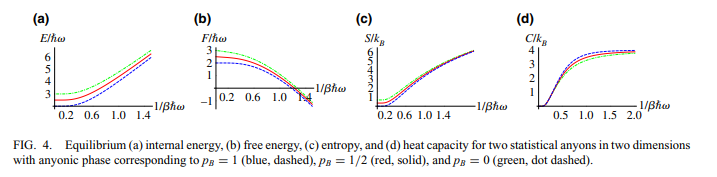
\includegraphics[width=100mm]{fig4.png}
  \caption{2次元統計エニオンの熱力学量}
  \end{center}
\end{figure}

\subsubsection{2次元統計エニオンの分配関数}
2次元調和ポテンシャル中の2つの統計エニオンのハミルトニアンは、

\begin{align}
  H_{SA,2D} = \frac{1}{2m}(p_{x_1}^2+p_{y_1}^2+p_{x_2}^2+p_{y_2}^2)+\frac{1}{2}m\omega^2(x_1^2+y_1^2+x_2^2+y_2^2)
\end{align}

となる。
ここで、$x_1,y_1$は粒子1の位置座標であり、$x_2,y_2$は粒子2の位置座標である。1次元統計エニオンの場合には、粒子1の座標を$x$,粒子2の座標を$y$としていた事に注意。

このハミルトニアンのもとで発展するエニオンのN個のペアの分配関数は、1次元のときと同様に、

\begin{align}
  Z_{SA,2D} = \mathrm{Tr}[\mathrm{e}^{-\beta H_{SA,2D}}] = \prod_{j=1}^N\int dx_{1j}\int dy_{1j} \bra{x_{1j}y_{1j}x_{2j}y_{2j}}\mathrm{e}^{-\beta H_j}\ket{x_{1j}y_{1j}x_{2j}y_{2j}}
\end{align}

である。粒子数表示のアイデンティティ

\begin{align}
  \sum_{n_1^{(j)},n_2^{(j)}=0}^{\infty}\ket{n_{1x},n_{1y},n_{2x},n_{2y}}\bra{n_{1x},n_{1y},n_{2x},n_{2y}}=1
\end{align}

を挟むことによって、位置表示の波動関数$\Psi_{SA,2D}(x_{1j},y_{1j},x_{2j},y_{2j})=\braket{x_{1j}y_{1j}x_{2j}y_{2j}}{n_{1x},n_{1y},n_{2x},n_{2y}}$を用いて、

\begin{align}
  Z_{SA,2D} &= \prod_{j=1}^N\int dx_{1j}\int dy_{1j}\int dx_{2j}\int dy_{2j} \sum_{n_{1x}^{(j)},n_{1y}^{(j)},n_{2x}^{(j)},n_{2y}^{(j)}} \sum_{m_{1x}^{(j)},m_{1y}^{(j)},m_{2x}^{(j)},m_{2y}^{(j)}}\\
   &\,\,\,\,\times|\Psi_{SA,2D}(x_{1j},y_{1j},x_{2j},y_{2j})|^2 \braket{m_{1x},m_{1y},m_{2x},m_{2y}}{n_{1x},n_{1y},n_{2x},n_{2y}} \\
\end{align}

となる。

\begin{align}
  \braket{m_{1x},m_{1y},m_{2x},m_{2y}}{n_{1x},n_{1y},n_{2x},n_{2y}}=\delta_{m_{1x},n_{1x}}\delta_{m_{1y},n_{1y}}\delta_{m_{2x},n_{2x}}\delta_{m_{2y},n_{2y}}
\end{align}

なる直交条件は、$\sum$をひとつにする。
$\prod$と$\sum$を除いた形で、分配関数は

\begin{align}
  \int dx_{1j}\int dy_{1j}\int dx_{2j}\int dy_{2j}|\Psi_{SA,2D}(x_{1j},y_{1j},x_{2j},y_{2j})|^2
\end{align}

となる。ここで、全系の波動関数は

\begin{align}
  \Psi_{SA,2D}(x_{1j},y_{1j},x_{2j},y_{2j})=\frac{1}{\sqrt{(1+2\delta_{m_{1x},n_{1x}}\delta_{m_{1y},n_{1y}}\delta_{m_{2x},n_{2x}}\delta_{m_{2y},n_{2y}})}}\left(\frac{m\omega}{\pi\hbar}\right)^2 \notag \\
  \times\mathrm{e}^{\frac{m\omega}{2\hbar}(x_{1j}^2+y_{1j}^2+x_{2j}^2+y_{2j}^2)} \left[\psi_{n1}(x_{1j},y_{1j})\psi_{n2}(x_{2j},y_{2j})+\mathrm{e}^{i\pi\nu_j}\psi_{n1}(x_{2j},y_{2j})\psi_{n2}(x_{1j},y_{1j})\right]^2
\end{align}

である。統計エニオンとしてみなすには

\begin{align}
  \mathrm{e}^{i\pi\nu_j}=\mathrm{e}^{i\pi\Theta(j-N_B+1)}
\end{align}

であることが必要である。2次元の1粒子波動関数は

\begin{align}
  \psi_n(x,y)=\frac{1}{\sqrt{2^n n!}}\left(\frac{m\omega}{\pi\hbar}\right)^{1/2}\mathrm{e}^{\frac{m\omega}{2\hbar}(x^2+y^2)}H_n\left(\sqrt{\frac{m\omega}{\hbar}}x\right)H_n\left(\sqrt{\frac{m\omega}{\hbar}}y\right)
\end{align}

である。$\sqrt{\frac{m\omega}{\hbar}}x=x\,(yも同様)$と置いて、これを用いると、

\begin{align}
  |\Psi_{SA,2D}(x_{1j},y_{1j},x_{2j},y_{2j})|^2&=\frac{1}{2^{n_1+n_2}n_1!n_2!}\left(\frac{m\omega}{\pi\hbar}\right)\times \mathrm{e}^{-(x_1^2+y_1^2+x_2^2+y_2^2)}\notag\\
  & \times[H_{n1}^2(x_1)H_{n1}^2(y_1)H_{n2}^2(x_2)H_{n2}^2(y_2)+2\mathrm{e}^{i\pi\nu_j}H_{n1}(x_1)H_{n_1}(y_1)\notag\\
  & \times H_{n2}(x_2)H_{n2}(y_2)H_{n1}(x_2)H_{n1}(y_2)H_{n2}(x_1)H_{n2}(y_1) \notag\\
  & +\mathrm{e}^{2i\pi\nu_j}H_{n1}^2(x_2)H_{n1}^2(y_2)H_{n2}^2(x_1)H_{n2}^2(y_1)] 
\end{align}

となる。エルミート多項式の直交性を利用することで、

\begin{align}
  Z_{SA,2D} &=\int dx_{1j}\int dy_{1j}\int dx_{2j}\int dy_{2j}|\Psi_{SA,2D}(x_{1j},y_{1j},x_{2j},y_{2j})|^2 \\
  &= \prod_{j=1}^N \sum_{n_{1x}^{(j)},n_{1y}^{(j)},n_{2x}^{(j)},n_{2y}^{(j)}=0}^{\infty}\frac{1}{4}\mathrm{e}^{-\beta\hbar\omega(n_{1x}^{(j)}+n_{1y}^{(j)}+n_{2x}^{(j)}+n_{2y}^{(j)}+2)}\notag\\ 
  &\times \left(\mathrm{e}^{-i\pi\nu_j}\delta_{n_{1x}^{(j)},n_{1y}^{(j)},n_{2x}^{(j)},n_{2y}^{(j)}}+2+\mathrm{e}^{i\pi\nu_j}\delta_{n_{1x}^{(j)},n_{1y}^{(j)},n_{2x}^{(j)},n_{2y}^{(j)}}\right)  \notag\\
\end{align}

となる。階段関数で積を分け、大きい$N$に対して、$p_B$は粒子のペアがボソン的な対称性を持つ確率であることを考慮すると、

\begin{align}
  Z_{B,2D}&=\prod_{j=1}^{N_B}\sum_{n_{1x}^{(j)},n_{1y}^{(j)},n_{2x}^{(j)},n_{2y}^{(j)}=0}\frac{1}{2}\mathrm{e}^{-\beta\hbar\omega(n_{1x}^{(j)}+n_{1y}^{(j)}+n_{2x}^{(j)}+n_{2y}^{(j)}+2)}(1+\delta_{n_{1x}^{(j)},n_{1y}^{(j)},n_{2x}^{(j)},n_{2y}^{(j)}})\\
  Z_{F,2D}&= \prod_{j=N_B+1}^{N}\sum_{n_{1x}^{(j)},n_{1y}^{(j)},n_{2x}^{(j)},n_{2y}^{(j)}=0}\frac{1}{2}\mathrm{e}^{-\beta\hbar\omega(n_{1x}^{(j)}+n_{1y}^{(j)}+n_{2x}^{(j)}+n_{2y}^{(j)}+2)}(1-\delta_{n_{1x}^{(j)},n_{1y}^{(j)},n_{2x}^{(j)},n_{2y}^{(j)}})
\end{align}

となる。

\subsection{2次元トポロジカルエニオン}
2次元調和ポテンシャル中の2つのトポロジカルエニオンの分配関数について考える。
これは、topological aspects of low-dimensional systems , Anyons: Quantum Mechanics of particles with fractional Statisticsなどで導かれており、

\begin{align}
Z_{TA}=\frac{\mathrm{e}^{-\beta\hbar\omega(2+\nu)}+\mathrm{e}^{-\beta \hbar \omega (4-\nu)}}{(1-\mathrm{e}^{-\beta\hbar\omega})^2\mathrm{e}^{-4\beta\hbar\omega}}
\end{align}

となる。ここで、$\nu$はエニオンの位相である。
トポロジカルエニオンの分配関数は、フェルミオンとボソンの関数として表すことはできないことに注意。
これは、トポロジカルエニオンの波動関数の複雑性を増している。
2粒子エニオン系のエニオンの位相は相対運動の角運動量のシフトと見ることができる。[43]\\
しかし、(ブレイド群ベースのトポロジカルエニオンに限って)位相は回転方向に依存するという事実は、多価の波動関数であることを導く[51]。
位相に依存する波動関数の二つの分岐は、上の波動関数の分子にあらわれている(わからない)。\\
分配関数がわかったので、平衡系の熱力学量を計算することができる(付録B)。

\begin{figure}[htbp]
  \begin{center}
  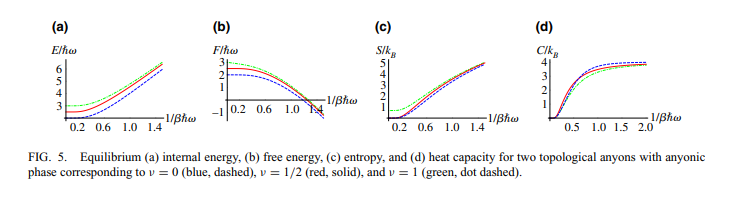
\includegraphics[width=100mm]{fig5.png}
  \caption{トポロジカルエニオンの熱力学量}
  \end{center}
  \end{figure}

トポロジカルエニオンのエントロピーはゼロ温度極限で0に向かう。
これは統計エニオンの結果とは対照的である。(まだこれは正しいかわからない。)
これは、$\nu=1$(これは純粋なフェルミオンである)を除いたすべての$\nu$で、基底状態がひとつであるからである。
あと違うのは、比熱のふるまいである。低温において、トポロジカルエニオンの比熱はフェルミオンとボソンの比熱より高い。
この比熱のふるまいを除くと、統計エニオンとトポロジカルエニオンの熱力学量のふるまいは、フェルミオン極限とボソン極限のあいだに$p_B=1/2$の線が存在しているという点において似ているといえるだろう。
基底状態では、波動関数のふたつの枝(波動関数は多価関数になるらしいので、そのことだと思う)に対応したエネルギー固有値はフェルミオン極限においてのみ一致する。
しかし、有限温度においては、トポロジカルエニオンがハードコアであるという本質は熱力学量をフェルミオニック極限に近づける。

\begin{figure}[htbp]
  \begin{center}
  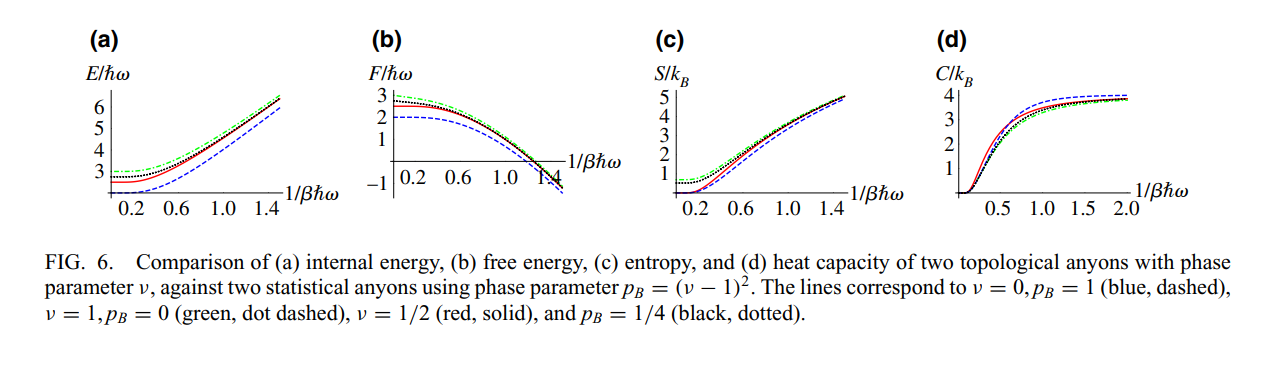
\includegraphics[width=100mm]{fig6.png}
  \caption{$p_B=(\nu-1)^2$のもとでの統計エニオン、トポロジカルエニオンの熱力学量}
  \end{center}
  \end{figure}


トポロジカルエニオンの比熱のユニークなふるまいも似た事情による。
ゼロ温度極限では、トポロジカルエニオンの内部エネルギーは、ボソニックな基底状態とフェルミオニックな基底状態の中間ほどの内部エネルギーに内挿される。
一方、高温では、フェルミオニックな値に近づく。
hogehoge(あといろんな値の説明があるけどこれはまたあとで)

\subsection{熱力学的等価性}
統計エニオンの枠組みをもって、トポロジカルエニオンのゆたかなふるまいを説明できるか?
トポロジカルエニオンのパラメータ$\nu$と、統計エニオンのパラメータ$p_B$の間の関係は、分配関数を等しいとおくことにより

\begin{align}
p_B = \frac{\ln{\cosh\left[(\nu-1)\beta\hbar\omega\right]}}{\ln\left(\cosh(\beta\hbar\omega)\right)}
\end{align}

これをみると、$p_B$の複雑なふるまいは、温度と周波数の関数でもあるからということによるとみることができる。
上式の高温極限をとると、もっとシンプルな形になる:

\begin{align}
p_B=(\nu-1)^2
\end{align}

これをみると、この極限のもとでは、$\nu=0,1$はそれぞれ、ボソン極限、フェルミオン極限であるとみれる。
つまり、さきほどの、GESパラメータと、第2ビリアル係数を使ったトポロジカルエニオンの位相の間の関係もまた2次多項式である(?)[12]。
この$p_B$をもちいて熱力学量を計算すると、統計エニオンとトポロジカルエニオンが同一になったときの関係を得る。
統計エニオンを用いたトポロジカルエニオンの熱力学的性質を真似する能力は、実験的立場からみると、より問題を複雑にする。
2次元物質内でトポロジカルエニオンを操作し、検出することはむずかしいため、トポロジカルエニオンの熱力学を証明することも難しい。
統計エニオンは、トポロジカルエニオンの熱力学的操作のテストモデルとして機能するかもしれない。

\section{可逆エニオンエンジン}
統計的エニオンと位相的エニオンの平衡熱力学的振る舞いを確立したところで、私たちはこれらのエニオンが熱機関においてどのように振る舞うかについての探究を続ける。
平衡熱力学においては、どんな熱機関の最高効率も、Carnot効率にバウンドされる。
しかし、この効率は、無限に遅い準静的過程極限において、ゼロパワーアウトプットにより達成される。
もっと実践的な使い方をするため、可逆熱力学という枠組みを用いて、CurzonとAhlbornにより"最高動力効率(Efficency at maximum power,EMP)"の概念は導入された。
CurzonとAhlbornは、可逆CarnotエンジンのEMPは

\begin{align}
\eta_{CA}=1-\sqrt{\frac{T_C}{T_H}}
\end{align}

であることを発見した[98,M. H. Rubin, Optimal configuration of a class of irreversible heat engines. i, Phys. Rev. A 19, 1272 (1979).]。
ここで、$T_C,T_H$は低温、高温の熱浴の温度である。\\

可逆熱力学では、着目系(以降、システム)は常に局所熱平衡であるとみなされる。
しかし、環境も含めた大域熱平衡が達成されないほどの速さで起こるダイナミクスは考える。
これは、結果として、ローカルには可逆で、グローバルには不可逆であることになる。

以下、エンジンを構成するシステムを動作媒体と呼ぶことにする。

量子Ottoエンジンのパフォーマンスは、ストロークのプロトコルや動作媒体に依存し、とくに、EMPについては、作動媒体の基本的な関係の形できまる。
[122]によると、1粒子が作動媒体である可逆量子OttoエンジンのEMPは、Curzon-Ahlborn効率(以下、CA効率)を超えられる。
これはすなわち、可逆熱力学という枠組みの中では、CarnotサイクルよりもOttoサイクルの方が効率が良くなりうるということを示唆しているのではないだろうか?(まだ確証はないが)\\
したがって、そのようなエンジンの動作における量子統計の役割を検討することは興味深いことである。

[122]で構築されたメソッドを追って分析してみる。
1次元調和ポテンシャル中の2つのエニオンが動作媒体であることを考えよう。
そのエニオンはハミルトニアン 

\begin{align}
  H=\frac{p_1^2+p_2^2}{2m}+\frac{1}{2}m\omega^2(x_1^2+x_2^2)
\end{align}

のもとで時間発展する。
$\omega$は時間に依存しない。

\subsection{可逆熱力学の枠組みでのOttoサイクルの一般論}
Ottoサイクルは、4つのステップで構成される。可逆過程を考えているので、等エントロピー過程は断熱過程とみなせる。

\begin{figure}[htbp]
  \begin{center}
  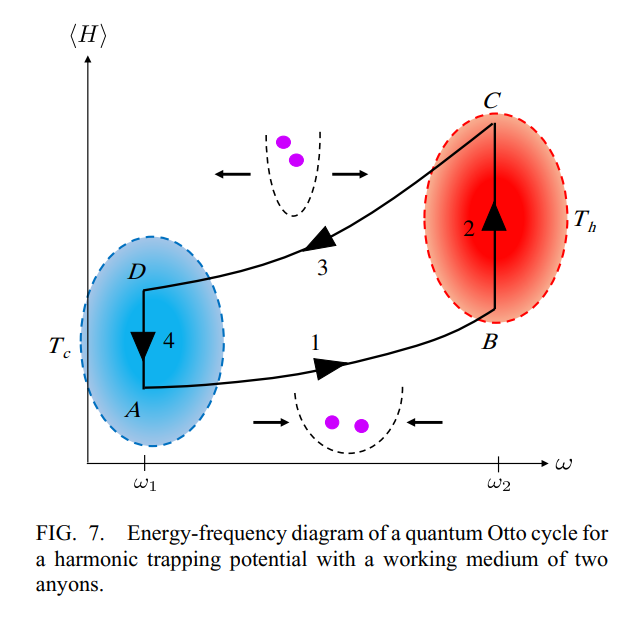
\includegraphics[width=100mm]{fig7.png}
  \caption{Ottoサイクル}
  \end{center}
  \end{figure}

\begin{enumerate}
  \item 断熱圧縮\\
  ストロークの間、作動媒体はエントロピーを保ち、熱を環境と交換しない。このとき、熱力学第一法則$\Delta E=Q+W$を用いる(システムのエネルギー変化を$\Delta E$、環境からシステムに入ってくる熱を$Q$、環境からシステムになされる仕事を$W$とする、システムに着目した形の第1法則。)と、
  \begin{align}
    W_{\text{comp}}=E(T_B,\omega_2)-E(T_A,\omega_1)
  \end{align}
  である。\\
  \item 等積加熱\\
  このストロークの間では、外部からコントロールされた仕事のパラメータを一定に保つ、結果として、システムは仕事をされない。
  第一法則を用いると、
  \begin{align}
  Q_h=E(T_C,\omega_2)-E(T_B,\omega_2)
  \end{align}
  となる。
  可逆性という条件を思い出すと、このストロークの間、作動媒体は高温のリザバーと完全に熱平衡化しない。
  すなわち、$T_B\leq T_C \leq T_h$である。
  動作媒体の性質に依存するというこのストロークの間、温度変化はFourierの法則にしたがう:
  \begin{align}
    \frac{dT}{dt}=-\alpha_h \left[T(t)-T_h\right]
  \end{align}
  ここで、$\alpha_h$は動作媒体の熱容量と熱伝導率により定まる定数である。\\
  \item 断熱膨張\\
  圧縮過程とまったく同じ手続きにより、断熱的に膨張させる。
  第一法則は
  \begin{align}
    W_{\text{exp}}=E(T_D,\omega_1)-E(T_C,\omega_2)
  \end{align}
  となる。\\
  \item 等積冷却\\
  等積加熱のときと同様の手続きにより、体積を保ったまま冷却する。
  第一法則は
  \begin{align}
  Q_C=E(T_A,\omega_1)-E(T_D,\omega_1)
  \end{align}
  温度変化はFourierの法則にしたがう:
  \begin{align}
    \frac{dT}{dt}=-\alpha_c \left[T(t)-T_C\right] 
  \end{align}
  ここで、$T_D > T_A \geq T_C$である。
\end{enumerate}

エンジンの効率は、システムが受け取った熱と、システムが環境にした正味の仕事の比で定義される:
\begin{align}
\eta=-\frac{W_{\text{comp}}+W_{\text{exp}}}{Q_h}
\end{align}
全体に負符号がついているのは、仕事をシステムから環境への仕事で定義したためである。

パワーアウトプットは、合計の仕事とサイクルの時間の比で定義される:

\begin{align}
P=-\frac{W_{\text{comp}}+W_{\text{exp}}}{\gamma (\tau_h + \tau_c)}
\end{align}

ここで、$\tau_h ,\tau_c$は加熱ストローク、冷却ストロークの時間であり、$\gamma$は等積過程を表すためのパラメータである。
すなわち、全サイクル時間を$\tau$として、

\begin{align}
\tau=\gamma(\tau_h+\tau_c)
\end{align}

であるだろうと思われる。

\subsection{1次元統計エニオンエンジン}
1次元統計エニオンの熱力学量を、Ottoサイクルの第一法則の式に入れることで、Ottoサイクルのパワーを計算する。
断熱過程においては、エントロピーは等しいので

\begin{align}
S(T_A,\omega_1) = S(T_B,\omega_2)\\
S(T_C,\omega_2) = S(T_D,\omega_1)
\end{align}

なる条件が満たされる。
エントロピーの表式を考えると、

\begin{align}
T_A\omega_2=T_B \omega_1  \\
T_C\omega_2=T_D \omega_1
\end{align}

である。

温度変化はFourierの法則にしたがうため、方程式を解いて

\begin{align}
T_C-T_h=(T_B-T_h)\mathrm{e}^{-\alpha_h \tau_h}\\
T_A-T_c=(T_D-T_c)\mathrm{e}^{-\alpha_c \tau_c}
\end{align}

ここで、$\tau_h,\tau_c$は加熱、冷却ストロークの時間である。
これらの方程式を用いて、Ottoサイクルの効率は

\begin{align}
\eta = 1 - \kappa
\end{align}

となる。
ここで、$\kappa \coloneq \omega_1/\omega_2 $ で定義され、圧縮比とよぶ。
この効率は、古典的な可逆Ottoエンジンと1粒子量子Ottoエンジンで同じであり、完全に作動媒体の量子統計的性質から独立している。
EMPを計算するにあたり、パワーを計算すると、

\begin{align}
P=\frac{(1-\kappa)\hbar\omega_2}{\gamma(\tau_h+\tau_c)}[3\coth(\Gamma)-3\coth(\Lambda)+\csch(\Gamma)-\csch(\Lambda)]
\end{align}

となる。ここで

\begin{align}
\Gamma=\frac{\kappa\hbar\omega_2 (\mathrm{e}^{\alpha_c\tau_c+\alpha_h\tau_h}-1)}{k_B T_h \left[\kappa T_h (\mathrm{e}^{\alpha_h \tau_h}-1)\mathrm{e}^{\alpha_c \tau_c}+T_c(\mathrm{e}^{\alpha_c \tau_c}-1)\right]}\\
\Lambda=\frac{\kappa\hbar\omega_2 (\mathrm{e}^{\alpha_c\tau_c+\alpha_h\tau_h}-1)}{k_B T_h \left[\kappa T_h (\mathrm{e}^{\alpha_h \tau_h}-1)+T_c(\mathrm{e}^{\alpha_c \tau_c}-1)\mathrm{e}^{\alpha_c \tau_c}\right]}\\
\end{align}

である。
結局、可逆アウトプットパワーは1次元統計エニオンの量子統計的な性質に依存しないことがわかる。
これはref[121]での結果と一貫性がある。
[127]は、作動媒質のボソニックまたはフェルミオン的性質に起因する一次元調和量子Ottoエンジンの性能の違いが、非平衡での性能の特徴であることを示している。
可逆操作であるという条件が与える、一般化排他統計の唯一の影響は、圧縮ストロークでの仕事を$p_B \hbar (\omega_1 - \omega_2)$だけ、膨張ストロークでの仕事を$p_B \hbar (\omega_2 - \omega_1)$だけシフトさせることである。
それゆえ、トータルの仕事としてこれらを足すと、そのシフトの効果はキャンセルされて見えなくなる。

$\Gamma=\Lambda$のとき、$P=0$となることがわかる。
これは、$\kappa \to {T_c}/{T_h}$ のとき達成されることがわかる。
この極限はCarnot効率での準静的操作に対応するため、これは物理的直感と一致する。
パワーアウトプットが正であり、サイクルがエンジンとして機能する(これはどういう条件?)とき、$\Gamma < \Lambda$である。

EMPを求めるため、圧縮率を変え、パワーを数値計算で最大化する。
1次元統計エニオンにおける、熱浴の温度の比の関数で見たEMPのグラフをFIG8に示す。

\begin{figure}[htbp]
  \begin{center}
    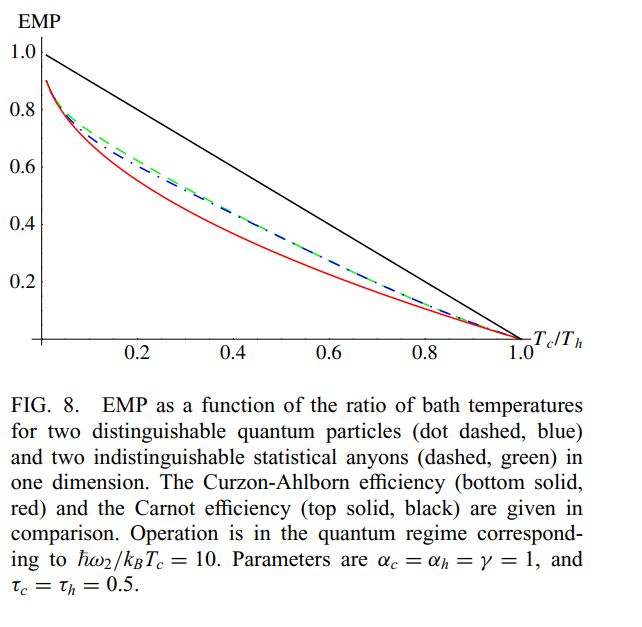
\includegraphics[width=100mm]{fig8.png}
    \caption{1次元統計エニオンエンジンのEMP}
  \end{center}
\end{figure}

驚くべきことに、EMPはエニオニックな位相には依存せず、粒子が区別できるかどうかに依存する。
粒子が区別できる場合というのは、2粒子が空間的に離れており、粒子の波動関数のオーバーラップが無視できるほど小さく、交換力からくるふるまいを考えなくてよいときのことである。
実験的には、2つの区別可能な粒子からなるエンジンは、ラボを挟んで互いに位置する2つの別個の単一粒子エンジンの共同出力と等価であると考えることができる。

温度比が低いとき、粒子が区別できるエンジンのEMPは、区別できないエンジンのEMPを上回る。
FIG8では、低温度比帯では緑線が青線を超えるということである。
また、両者のEMPはCA効率を超えるというRef[121]の結果を再現している。

\subsection{2次元統計エニオンエンジン}
ストレートフォワードに、2次元統計エニオンエンジンのEMPを計算することができる。
違う点は、熱力学量は$p_B$に依存することである。
これはパワーに影響を与える。
あとでほかの文を読む。

\subsection{2次元トポロジカルエニオンエンジン}
2次元トポロジカルエニオンエンジンは、以前求めた分配関数から始めることができる。
これは結果として、






\section{disscussion}

\subsection{統計エニオンの実験をしたらどうなるか?}
HOM効果の拡張としての統計エニオンの作成は、2つのポート(片方はパスの長さを変えている)から2つのポートへの光子の移動により行われるのであった。
そこから波動関数を考え、分配関数を考え、熱力学量を計算した。
バンチングのあと、統計エニオンはどちらかのポートにいるはずである。
パスの長さを変えただけなので、とくに粒子のチャージやスピンなどに影響は与えていない。
よって、見た目は、単なる光の集まりであると予想される。
この光子の集団を古典的に見た場合、得られた位相は、古典的な波動の位相だとみてよいのか?
$\to$ これはよくない。
なぜなら、統計エニオンの位相は、粒子の入れ替えによって得られた位相であるから、古典的な波動の位相とは異なるものである。

\subsection{統計エニオンの熱力学量はどのように計測するか?}
$\ket{a},\ket{b}$から出ていった光子は、すで統計エニオンとなる。
はじめに、エンタングルしている光子を準備する段階ではエニオンではない。導波管を通っている間に統計エニオンになると考えてよいのだろうか?
この統計エニオンに対する熱力学量の計算は、ハミルトニアンを用いて行われた。\\
調和ポテンシャルはどこで作っているのか?\\
反射して、$\ket{c},\ket{d}$に入ったあとで、どこかに集めて、そこで調和ポテンシャルと合わせる?
熱力学量は平衡系で考えているので、なにかケースの中に集めてそれを逆温度$\beta$の熱浴と接しさせて熱力学量を測定しているのだろうか。
普通の光子気体と同じように熱力学量を計算しているとみてよいだろうか。

\subsection{エニオンエンジンの速度とパワーのトレードオフ関係}
これを計算してみたい。\\
Y.Hasegawa TUR in quantum system\\
https://link.aps.org/doi/10.1103/PhysRevResearch.2.022044\\
https://journals.aps.org/prl/abstract/10.1103/PhysRevLett.126.010602\\
TURに関しては、N.Shiraishi "An Introduction to Stochastic Thermodynamics"の16章も参照した方がよい。

\subsection{トポロジカルエニオンと統計エニオンの一致}
これも考えてみたい。
統計エニオンを2次元系に押し込めてみる。
この統計エニオンをトポロジカルエニオンにしてみたらどうなるだろうか?
統計エニオンは光子から作るため、どのようにトポロジカルエニオンにするかを考えなければいけない。

\subsection{エニオンエンジンの効率とパワーのトレードオフ関係}
https://www.mdpi.com/1099-4300/23/9/1149\\
https://journals.aps.org/pre/abstract/10.1103/PhysRevE.85.031145\\
https://www.nature.com/articles/s41467-017-01991-6\\
https://journals.aps.org/prresearch/abstract/10.1103/PhysRevResearch.4.013157\\
https://link.aps.org/doi/10.1103/PhysRevE.106.024137\\



\section{Appendix}
\subsection{可逆熱力学について}
ここでは、エンジンの章で考えた可逆熱力学についてまとめてみる。
まず、可逆熱力学はどのような立場なのかをまとめる。
ここでの定義はN. Shiraishi, "An Introduction to Stochstic Thermodynamics",p.298に従っているため、多少本文と異なる。

\begin{itembox}[l]{\textbf{Def.可逆熱力学}}
可逆熱力学は、温度$T$の熱浴に接した注目系(以下、システムと呼ぶ)の等温過程のことで、以下の性質を満たす。
\begin{enumerate}
  \item システムは常に熱平衡である。
    システムが熱平衡にあるため、システムの温度$T'$は定義される。
    ここで、$T\neq T'$であってもよい。
  \item システムと熱浴の間のエネルギー交換はFourierの法則に従う:
    \begin{align}
      J_Q=\kappa(T-T')
    \end{align}
    ここで、$J_Q$はシステムから熱浴への熱流(ほとんど熱のようなもの)、$\kappa_C$は熱コンダクタンスである。
  \item システムの温度$T'$はシステムの平衡熱力学から定める。すなわち、システムの内部エネルギー$E$、体積$V$、粒子数$N$から決める。
\end{enumerate}
\end{itembox}

熱コンダクタンス$\kappa_C$は熱伝導率$\kappa$と、エンジンと熱浴の接触面積$A$を用いて

\begin{align}
  \kappa_C=\kappa A
\end{align}

により定められる。







\end{document}

